\documentclass[a4paper,11pt]{article}
\usepackage[UKenglish]{babel}
\usepackage[table]{xcolor}
\usepackage{graphicx}
\usepackage{courier}
\usepackage{color}
\usepackage{array}
\usepackage{pstricks}
\usepackage{parskip}
\usepackage[bottom]{footmisc}
\usepackage{fancyhdr}
\usepackage{multirow}
\usepackage{longtable}
% the hyperref package must always be the last package to be included
\usepackage[pdftex,
            pdfusetitle,
            pdfsubject={Technical Reference Manual for dastaZ80 homebrew computer},
            pdfkeywords={Z80, homebrew computer, Operating System, OS, programmer, technical, reference, manual}
        ]{hyperref}

\hypersetup{
    colorlinks = true,
    linkcolor = blue,
    anchorcolor = blue,
    citecolor = blue,
    filecolor = blue,
    urlcolor = blue
}

\setlength\parindent{0pt}

\begin{document}
    \pagestyle{empty}
    % ==========================================================================
    % Cover page
    % ==========================================================================
    \begin{pspicture}(8.5,11)
        \rput[b](3.5,8){
            \parbox{7in}{
                \begin{flushright}
                    \Huge\bfseries\sffamily dastaZ80 Mark I\\ Technical Reference Manual
                \end{flushright}
            }
        }
        \uput[0](0,0){\color{blue}\rule{7in}{0.5ex}}
    \end{pspicture}
    \title{dastaZ80 Technical Reference Manual}
    \author{David Asta}
    \date{11 October 2022}

    \pagebreak
    % ==========================================================================
    % Header & Footer
    % ==========================================================================
    \pagestyle{fancy}
    \fancyhf{}
    \fancyhead[R]{dastaZ80 Mark I Technical Reference Manual}
    % ==========================================================================
    \section*{Disclaimer}
    % ==========================================================================
    The products described in this manual are intended for educational purposes,
    and should not be used for controlling any machinery, critical component in
    life support devices or any system in which failure could result in personal
    injury if any of the described here products fail.
    
    These products are subject to continuous development and improvement. All
    information of a technical nature and particulars of the products and its
    use are given by the author in good faith. However, it is acknowledged that
    there may be errors or omissions in this manual. Therefore, the author
    cannot accept any liability for any loss or damage arising from the use of
    any information or particulars in this manual.

    % ==========================================================================
    \section*{Licenses}
    % ==========================================================================
    \small
    \textbf{Hardware} is licensed under the \textbf{Creative Commons
    Attribution-ShareAlike 4.0 International License}
    
    \hspace{1cm}http://creativecommons.org/licenses/by-sa/4.0/
    
    \textbf{Software} is licensed under \textbf{The MIT License}
    
    \hspace{1cm}https://opensource.org/licenses/MIT
    
    \textbf{Documentation} is licensed under the \textbf{Creative Commons
    Attribution-ShareAlike 4.0 International License}
    
    \hspace{1cm}http://creativecommons.org/licenses/by-sa/4.0/

    \normalsize

    \hrulefill

    \textcopyright 2022 David Asta

    \pagebreak
    % ==========================================================================
    \section*{Document Conventions}
    % ==========================================================================
    The following conventions are used in this manual:

    \begin{center}
        \begin{tabular}{c m{9cm}}
            \hline
            \textbf{DEVICE} & Device names are displayed in bold all upper case 
            letters, and refer to hardware devices.\\
            \hline
            \texttt{Courier} & Text appearing in the \texttt{Courier} font 
            represents either an OS System Variable a Z80 CPU Register
            or a Z80 Flag. OS System Variables are identifiers for specific
            \textbf{MEMORY} addresses that can be used to read statuses and to
            pass information between routines or programs.\\
            \hline
            \texttt{0x14B0} & Numbers prefixed by 0x indicate an Hexadecimal value.
            Unless specified, memory addresses are always expressed in
            Hexadecimal.\\
            \hline
        \end{tabular}
    \end{center}

    The CompactFlash card is referred as \textbf{DISK}.

    The 80 column VGA output is referred as \textbf{CONSOLE}.
    
    The Operating System may be referred as DZOS, dzOS or simply OS.

    \textbf{MEMORY} refers to both \textbf{ROM} and \textbf{RAM}.

    \pagebreak
    % ==========================================================================
    \section*{Related Documentation}
    % ==========================================================================
    \hspace{1cm}{\LARGE dastaZ80 User's Manual}
    
    \hspace{1cm}{\LARGE dastaZ80 Programmer's Reference Guide}

    \hspace{1cm}{\LARGE https://github.com/dasta400/dzOS}

    \pagebreak
    % ==========================================================================
    \tableofcontents
    % ==========================================================================

    \pagebreak
    % ==========================================================================
    % Header & Footer
    % ==========================================================================
    \pagestyle{fancy}
    \fancyhf{}
    \fancyhead[R]{dastaZ80 Mark I Technical Reference Manual}
    \fancyfoot[R]{\thepage}
    \setcounter{page}{1}

    % ==========================================================================
    \section{Boards and Case}
    % ==========================================================================

    The final aim of dastaZ80 is to be a single board computer, but at the 
    moment I am making small \textit{module boards} so that I can test and 
    troubleshoot independently. Plus it allows me to easily upgrade and test
    (e.g. when I changed the serial board from a MC68B50 ACIA to a Zilog SIO/2).

    % ==========================================================================
    \subsection{Main board}
    % ==========================================================================

    This board is the heart of the computer, and contains the CPU chip, the 
    clock circuit, the reset circuit, the ROM chip, the RAM chip, the I/O
    decoding logic and the memory decoding logic.

    % ==========================================================================
    \subsubsection{CPU}
    % ==========================================================================

    The CPU is a Zilog Z80 (Z0840006PSC) NMOS 40-pin plastic DIP, rated at 6.17
    Mhz, but overclocked to 7.3728 MHz.

    The signals \textit{/INT}, \textit{/BUSREQ},\textit{/WAIT} and \textit{/NMI}
    are connected to 10K pull-up resistor

    % ==========================================================================
    \subsubsection{Clock circuit}
    % ==========================================================================

    This is the system clock, running at 7.3728 MHz, that drives the CPU and the
    SIO/2 Channels. It is a very simple circuit consisting of a crystal
    oscillator and a copule of resistors and ceramic capacitors.

    % ==========================================================================
    \subsubsection{Reset circuit}
    % ==========================================================================
    
    After power up, the CPU needs to be reset, through the \textit{/RESET}
    signal. When this signal is low for a minimum of three full clock cycles,
    the CPU resets the interrupt enable flip-flop, clears the Program Counter
    (\texttt{PC}), clears registers \texttt{I} and \texttt{R}, and sets the
    interrupt status to Mode 0. 

    In the dastaZ80, the reset circuit is a bit more complicated than the 
    typical reset circuit found in homebrew computers. The reason is that the
    VGA output is done with a LILYGO TTGO  VGA32 V1.4\footnote{An ESP32 board
    with a VGA output, that runs FABGL to provide an ANSI terminal.}, which
    needs a few seconds to initialise. So the reset is hold for 6.5 seconds, to
    allow the initialisation to finish,  and then reset the CPU and rest of
    devices.

    Using an NE555 timer running in monostable mode, the \textit{/RESET} signal
    is kept low a number of seconds that can be deduced with the formula: 
    $T = 1.1 * R2 * C2$. (e.g. $1.1 * 270000 (270K) * 0.000022 (22\mu F) = 
    6.534 seconds$).

    \begin{center}
        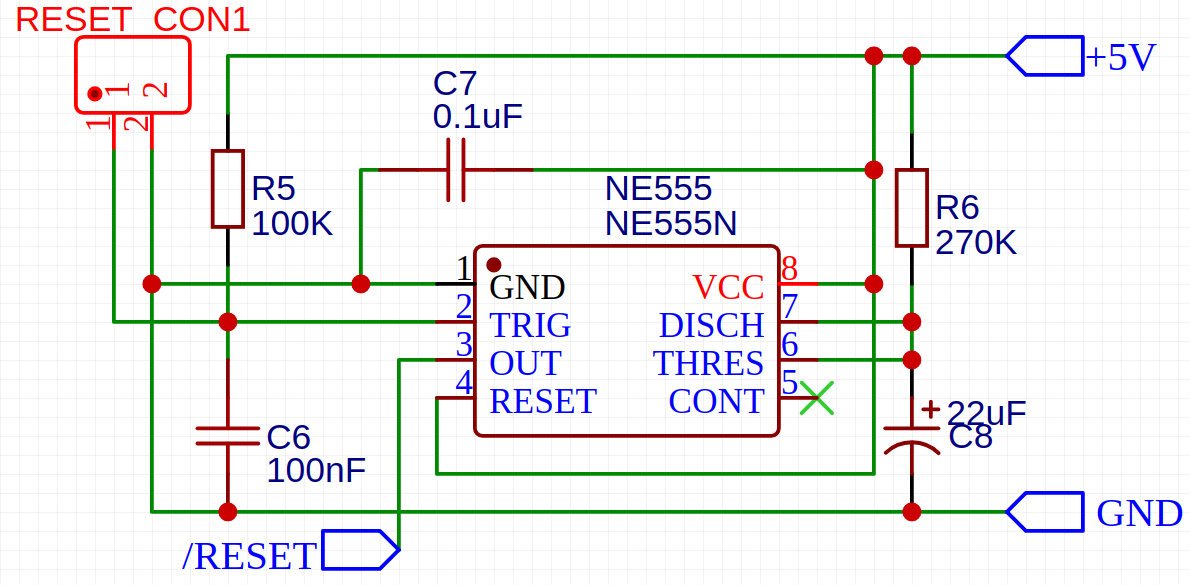
\includegraphics[scale=0.3]{dastaz80resetcircuit.png}
    \end{center}

    The \textit{RESET\_CON1} is connected to a push-button. R5 and C1 are used as 
    anti-debounce for the button.

    % ==========================================================================
    \subsubsection{ROM chip}
    % ==========================================================================

    The ROM chip is a Winbond W27E512 (64K x 8 bit) EEPROM (Electrically Erasable
    Programmable Read-Only Memory) 28-pin plastic DIP, mnounted on a ZIF (Zero
    Insert Force) socket for easy extraction/insertion for programming.

    The signal \textit{A15} is connected to \textit{+5V}, therefore is always
    high, meaning that the start address is \texttt{0x8000} and the ROM becomes
    a 32 KB ROM. This is not the start address that the CPU sees but rather the
    address where the ROM starts. The CPU will see it as \texttt{0x0000}.

    As the dzOS is 16 KB in size, I have divided the ROM into two 16 KB ROMs, 
    allowing to execute two different operating systems by selecting the start
    address (\texttt{0x8000} or \texttt{0xC000}) via a switch connected to the
    signal \textit{A14} of the ROM chip.

    When the switch is in the lower position, \textit{A14} is connected to 
    \textit{Ground}, thus start address \texttt{0x0000} starts at 
    \texttt{0x8000} in the ROM. When the switch is in the upper position, 
    \textit{A14} is connected to \textit{+5V}, thus start address is at 
    \texttt{0xC000}.

    The idea is to be able to use the computer with either dzOS or Digital 
    Research, Inc. CP/M. Of course, the CompactFlash will need to be changed
    for the specific operating system.

    % ==========================================================================
    \subsubsection{RAM chip}
    % ==========================================================================

    The RAM is an AS6C1008 (128K x 8 bit) CMOS SRAM 32-pin plastic DIP.

    As the Z80 can only address 65,536 bytes (64 KB), \textit{A16} on this chip
    is connected to \textit{Ground}, therefore it will always be low, and hence
    only 65,536 bytes (64 KB) are available.

    % ==========================================================================
    \subsection{Serial board}
    % ==========================================================================

    The serial board consists of a Zilog SIO/2 (Z84C4208PEG) CMOS 40-pin plastic
    DIP, rated at 8 MHz, that offers two independent full-duplex channels for
    data serial communication.

    Channel A is used for communication with the Keyboard Interface and the VGA
    Interface. The Transmit signal (\textit{TX}) of the Keyboard Interface is
    connected to the Receive signal (\textit{RX}) of the Channel A, and the 
    Transmit signal (\textit{TX}) of the Channel A is connected to the Receive
    signal (\textit{RX}) of the VGA Interface.

    The type of implementation allows for easy replacement of the keyboard and
    the screen output with any other serial terminal.

    Channel B is not used at the moment, but the aim is to add a MAX232 and a 
    RS-232 9-pin male connector to offer serial communication with other
    devices.

    Both channels are initialised for: 115,200 bps, 8N1

    % ==========================================================================
    \subsection{CompactFlash board}
    % ==========================================================================

    As I never soldered Surface Mount Device (SMD), for the CompactFlash board
    I chose to use the RC2014 Compact Flash Module which comes already with the
    CF card adaptor soldered.

    Nevertheless this module is rather simple and does not contain any kind of
    buffering, hence the module has to be connected very close to the CPU. For
    dastaZ80 I want to be able to swap CF cards, and therefore I need the card
    a bit far away from the Main Board. So I modified the RC2014 module to add
    a 74HCT245 (Octal bus transceiver).

    % ==========================================================================
    \subsection{Keyboard Interface}
    % ==========================================================================

    The keyboard I am using is a Acorn Archimedes A3010. The keyboard matrix is
    connected via its ribbon cable to a Teensy++ 2.0, which reads the status of
    the keys and sends the keystrokes via the Teensy serial pin to the SIO/2
    Channel A.

    A debouncing delay is applied to avoid the mechanical bouncing effect of
    keyboards, and keys are sent at a configurable (in the controller code)
    interval for as long as the key is pressed down.

    The interface sends ASCII values for all printable keys (i.e. alphabetical
    A to Z, numerical 0 to 9, and symbols lile !, @, \%, etc.). The rest of the
    keys are interpreted as special keys and special codes between 0x01 to 0x31
    are sent. With exception of the pound key, which sends the code 0x9C.

    \begin{center}
        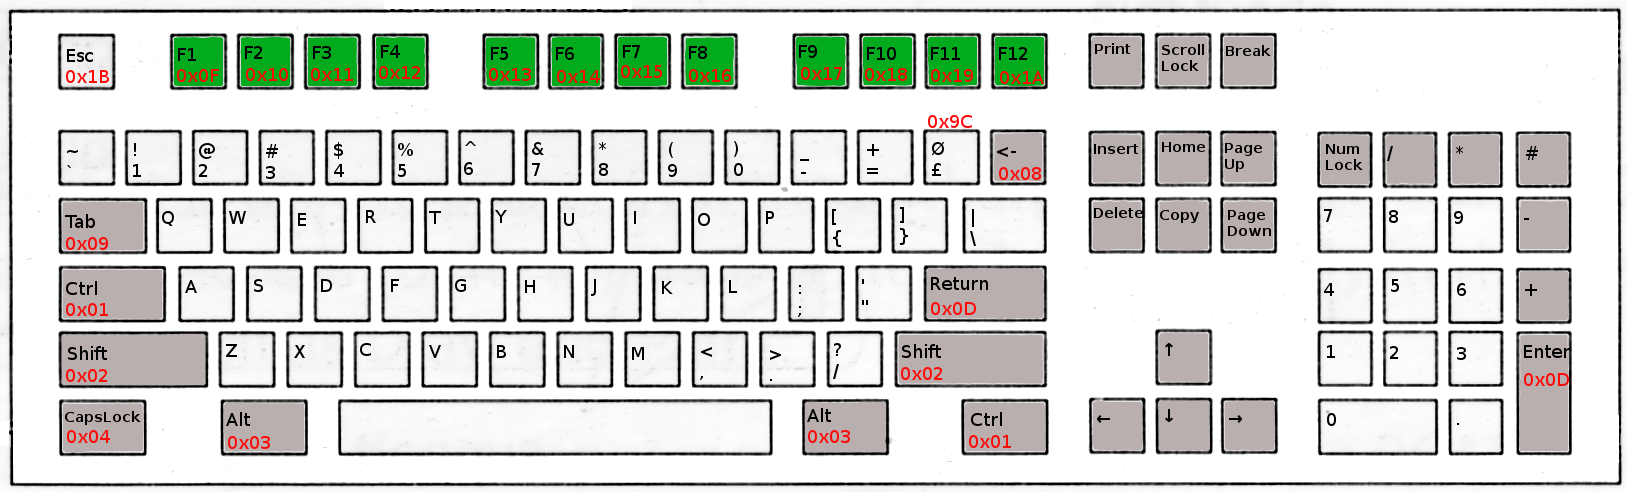
\includegraphics[scale=0.3]{a3010_kbd_layout.png}
    \end{center}

    % ==========================================================================
    \subsection{VGA Interface}
    % ==========================================================================

    The VGA output is achieved in a rather simple manner; the SIO/2 Channel A
    sends its output to a LILYGO TTGO VGA32 V1.4, which runs a very simple ANSI
    terminal emulator using the FabGL library.


    % ==========================================================================
    \subsection{Backplane}
    % ==========================================================================

    The backplane is where all the other boards are connected to. It consists
    of a single board with six double row 80-pin female connectors at 90 degrees
    angle.

    The connectors drive all CPU signals and the power (+5V and Ground).

    % ==========================================================================
    \subsection{Power Supply}
    % ==========================================================================

    The whole computer is powered via an external 12V/4A AC adaptor, which is 
    connected to an internal PSU5a (5V 3A Regulator in TO-220 form factor).

    The PSU5a output (5V) is connected diurectly to the backplane to supply 5V
    for all the boards, and also to an USB cable that powers the VGA32 board.

    % ==========================================================================
    \subsection{Computer Case}
    % ==========================================================================

    All the boards are inside an Acorn Archimedes A3010 all-in-one case that I
    had as spare.

    \begin{center}
        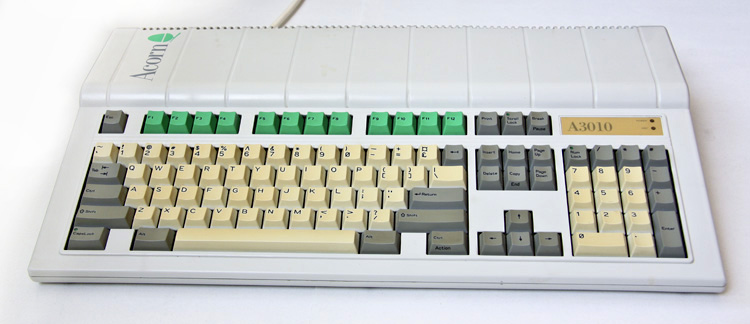
\includegraphics{acorn3010top.jpg}
    \end{center}

    The keyboard in the Acorn A3010 case is very PC-like, it has 12 function
    keys and LEDs for Caps Lock, Scroll Lock and Num Lock.

    The back of the case offers holes for connectors for: one DB-25 parallel, 
    one DB-9 serial, two DB-9 joysticks, one stereo jack, one VGA, one RF and
    ON/OFF switch.

    Also there is a hole in the left side for a reset button, and a disk drive
    bay at the right side.

    At the moment, only the ON/OFF switch, VGA connector and reset button are
    used.

    \pagebreak
    % ==========================================================================
    \section{I/O Decoding}
    % ==========================================================================

    The Z80 communicates with devices via the Address and Data buses. And then
    the signals \textit{/MREQ} (for memory devices) and \textit(/IORQ) (for I/O
    devices).

    To avoid bus contention\footnote{Bus contention occurs when all devices
    communicate directly with each other through a single shared channel
    (Address and Data buses), and more than one device attempts to place values
    on the channel at the same time.}, we need to enable each device one at a
    time.

    dastaZ80 uses a 74HCT138 (3-to-8 Line Decoder) to allow the CPU to enable
    I/O devices (non-memory devices). The outputs are enabled (low) when /MREQ
    is high, /IORQ is low and A7 is low (i.e. addresses below 0x80). This
    configuration gives 16 addresses for each device (e.g. \texttt{0x00} to
    \texttt{0x0F} for a device attached to output /Y0), for a total of 8 devices.

    \begin{tabular}{| c | c | c | c | c | m{4.5cm} | }
        \hline
        \rowcolor{lightgray}
        A6 & A5 & A4 & 74138 output & Addresses & Device\\
        \hline
        0 & 0 & 0 & /Y0 & \texttt{0x00} - \texttt{0x0F} & For future use\\
        \hline
        0 & 0 & 1 & /Y1 & \texttt{0x10} - \texttt{0x1F} & \textbf{DISK}
        (\texttt{0x10})\\
        \hline
        0 & 1 & 0 & /Y2 & \texttt{0x20} - \texttt{0x2F} & For future use\\
        \hline
        0 & 1 & 1 & /Y3 & \texttt{0x30} - \texttt{0x3F} & \textbf{ROM} Page
        (\texttt{0x38})\\
        \hline
        1 & 0 & 0 & /Y4 & \texttt{0x40} - \texttt{0x4F} & For future use\\
        \hline
        1 & 0 & 1 & /Y5 & \texttt{0x50} - \texttt{0x5F} & For future use\\
        \hline
        1 & 1 & 0 & /Y6 & \texttt{0x60} - \texttt{0x6F} & For future use\\
        \hline
        1 & 1 & 1 & /Y7 & \texttt{0x70} - \texttt{0x7F} & For future use\\
        \hline
    \end{tabular}
    
    \pagebreak
    % ==========================================================================
    \section{Memory Decoding}
    % ==========================================================================

    As dastaZ80 has a ROM chip and a RAM chip, the CPU has to decide from which 
    chip to read and to which chip to write. Actually, write operations are only
    applicable to the RAM chip.

    Also, dzOS\footnote{dzOS is the Operating System of dastaZ80.} resides in
    the ROM chip, but at boot the entire OS is copied into RAM so that it can be
    modified by the user. Hence, dastaZ80 needs a way to disable the ROM chip
    after the copy has finished.

    % ==========================================================================
    \subsection{Extra signals}
    % ==========================================================================

    To make the logic even more tight, dastaZ80 uses a 74HCT32 (Quad 2-Input or
    Gates) to create three new signals from signals comming from the Z80 CPU:

    \begin{itemize}
        \item \textit{/WR} or \textit{/MREQ} = \textit{/MEMWR}
        \item \textit{/RD} or \textit{/MREQ} = \textit{/MEMRD}
        \item \textit{/WR} or \textit{/MEMREG\_SEL}\footnote{Output /Y3 from the
        I/O Decoder 74HCT138} = \textit{/MEMREG}
    \end{itemize}

    % ==========================================================================
    \subsection{ROM Paging}
    % ==========================================================================

    The ROM paging (disable the ROM chip and enable the RAM chip for all memory
    related operations) is done with a 74HCT273 (Octal D-type Flip-Flop with
    Clear) acting as a external register, where the output 1 of this chip is 
    defined as \textit{/ROMPAGE}.

    When a 0 or a 1 is put into the register's input D0 and \textit{/MEMREG} 
    becomes high, then \textit{/ROMPAGE} signal becomes low or high.
    
    This 74HCT273 is identified in the circuit as \textit{MEMREGCFG}.
    
    % ==========================================================================
    \subsection{Putting all together}
    % ==========================================================================
    
    At power-on or after reset, the 74HCT273 is reset and all outputs are set to
    low, therefore \textit{/ROMPAGE} becomes low. From now on, when there is a
    memory read (\textit{/MEMRD} low) for an address lower than 0x4000
    (\textit{A14} and \textit{A15} low), the ROM chip is enabled
    (\textit{/ROM\_CE low}). When the address is equal or higher than 0x4000
    (\textit{A14} or \textit{A15} high), the RAM chip is enabled
    (\textit{/ROM\_CE} high).

    When there is an IO write (\textit{/IORQ} and \textit{/WR} low) to the any
    address from 0x30 to 0x3F, \textit{/MEMREG\_SEL} becomes low and therefore 
    \textit{/MEMREG} becomes low and \textit{MEMREG}\footnote{\textit{MEMREG} is
    an inverted signal of \textit{/MEMREG} done via a 74HCT04} becomes high. This
    (\textit{MEMREG} high) triggers the Flip-Flop on the 74HCT273, which takes
    whatever is at the inputs (CPU Data bus: \textit{D0}..\textit{D7}) and
    latches it to the outputs. Thus, if \textit{D0} contains a 1,
    \textit{/ROMPAGE} will go high and stay like that until \textit{MEMREG} goes
    high again. From now on, when there is a memory read (\textit{/MEMRD} low)
    \textit{/ROM\_CE} will be high independently of the address (\textit{A14}
    or \textit{A15}, low or high), thus only enabling the RAM chip.

    \pagebreak
    % ==========================================================================
    \section{Future Improvements}
    % ==========================================================================

    This are some ideas I have for improvements:

    \begin{itemize}
        \item \textbf{Dual video output}: the idea is to have the current VGA
                output as \textit{High Resolution} output, for high quality 
                80 column usage, and then add a TMS9918A VDP for 
                \textit{Low Resolution} 40 column graphics (e.g. games).
        \item \textbf{Sound Interface}: stereo sound output with an AY-3-8912.
        \item \textbf{Parallel Interface}: mainly for printer connection.
        \item \textbf{Dual Digital Joystick Port}: Allowing connection of two
                Commodore 64 compatible joysticks.
        \item \textbf{Cartridge Port}: allowing almost instantaneously load and
        access to programs stored in EEPROMs.
    \end{itemize}
\end{document}